\section{Tutorial - I2C, Debouncing and PWM}



Submit a single PDF (named correctly with STUDNUM1\_STUDNUM2\_Tut4.pdf) answering the following questions. If you pull from any sources, be sure to correctly cite them. 
\begin{enumerate}
    \item I2C\\
    I2C is a synchronous (a common clock signal is used to synchronise the data transfer) communication protocol. It requires only two bus line, SDA (data line) and SCL (Clock line). Each device connected on the bus is identified by its unique address.
    \begin{enumerate}
        \item Give the message structure for I2C protocol when master communicates with slave. [4] 
        \item Give 2 advantages of I2C over SPI? [2]
        \item Describe the start and stop conditions for I2C. [2]
        \item Draw a timing diagram showing a Master sending 0b11010101 to slave at address 0b1110000. [8]
    \end{enumerate}
    \item PWM\\
    The RPi doesn’t not have an onboard DAC in order to generate analogue voltages. Instead,  pulse width modulation (PWM) is used. PWM is a modulation technique used to get the average voltage output from a digital source.
    
            \begin{figure}[H]
            \centering
            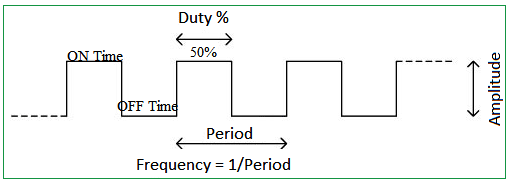
\includegraphics[width=0.8\columnwidth]{Figures/PWM.PNG}
            \caption{PWM parameters}
            \label{fig:my_PWM}
        \end{figure}
    
    \begin{enumerate}
        \item Why is that PWM in software on the Raspberry Pi is particularly ineffective/does not work? Hint: Make reference back to Real Time systems and requirements, paying attention to the operating system used on the Raspberry Pi [2]
        \item Explain the concept of persistence of vision, and why it can be useful in simplifying circuit designs. [2]
        \item What is the difference between PWM frequency and the duty cycle? [1] 
        \item Which parameter should you change when increasing the brightness on the LED? [1]
    \end{enumerate}
    \item Embedded Systems Good Practices
    \begin{enumerate}
        \item Why do we use pull up and pull down resistors? [2]
        \item Explain the difference between hardware debouncing and software debouncing, with an example of how you might implement each (i.e draw a circuit diagram and write a code snippet). [3]
        \item What is ``polling" in this context, and why is it better to use an interrupt over polling? [2]
    \end{enumerate}
\end{enumerate}